\documentclass[12pt]{article}
\usepackage{amsfonts, amssymb, amsmath, amsthm}
\usepackage[margin=1in]{geometry}
\usepackage{tikz}
\usetikzlibrary{patterns, decorations.pathreplacing, arrows.meta, 3d}

\pagestyle{myheadings}
\markright{Explainer: Rudin 4.7 --- Continuity Along Lines vs.\ at a Point\hfill}

\newcommand{\R}{\mathbb{R}}

\begin{document}

\begin{center}
    \textbf{\Large Continuous on Every Line $\neq$ Continuous at a Point}\\[0.5em]
    \large A visual guide to Rudin 4.7
\end{center}

\section{The Big Picture}

This problem shows a \textbf{surprising} fact: a function on $\R^2$ can be continuous along \emph{every} straight line through the origin, and yet \emph{not} be continuous at the origin. Lines don't ``see'' everything!

\begin{center}
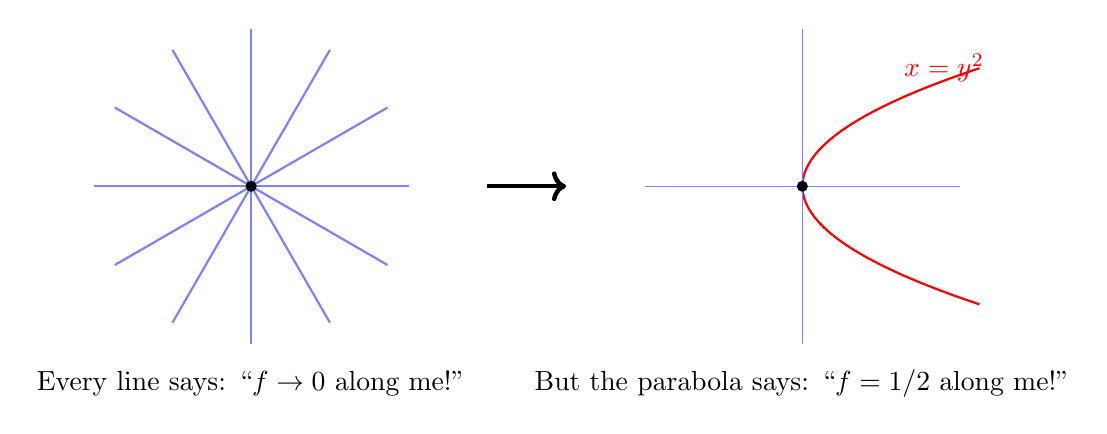
\begin{tikzpicture}[scale=1]
    % Lines through origin
    \foreach \angle in {0, 30, 60, 90, 120, 150} {
        \draw[blue!50, thick] ({-2*cos(\angle)}, {-2*sin(\angle)}) -- ({2*cos(\angle)}, {2*sin(\angle)});
    }
    \fill (0,0) circle (2pt);
    \node at (0, -2.5) {Every line says: ``$f \to 0$ along me!''};

    \draw[->, ultra thick] (3, 0) -- (4, 0);

    % Parabola
    \begin{scope}[xshift=7cm]
        \draw[red, thick, domain=-1.5:1.5, samples=50] plot ({\x*\x}, \x);
        \draw[blue!50] (-2, 0) -- (2, 0);
        \draw[blue!50] (0, -2) -- (0, 2);
        \fill (0,0) circle (2pt);
        \node[red] at (1.8, 1.5) {$x = y^2$};
        \node at (0, -2.5) {But the parabola says: ``$f = 1/2$ along me!''};
    \end{scope}
\end{tikzpicture}
\end{center}

\section{The Functions}

\[
f(x,y) = \frac{xy^2}{x^2 + y^4}, \qquad g(x,y) = \frac{xy^2}{x^2 + y^6}
\]
with $f(0,0) = g(0,0) = 0$.

\textbf{Notice the structure:} Both have the same numerator $xy^2$, but different denominators. The denominator controls how fast it grows, which determines boundedness and continuity.

\section{Part 1: Why is $f$ Bounded?}

\subsection{The AM-GM Trick}

The \textbf{AM-GM inequality} says: for non-negative numbers $a, b$,
\[
a + b \geq 2\sqrt{ab}
\]

Apply this to the denominator with $a = x^2$ and $b = y^4$:
\[
x^2 + y^4 \geq 2\sqrt{x^2 \cdot y^4} = 2|x| y^2
\]

\begin{center}
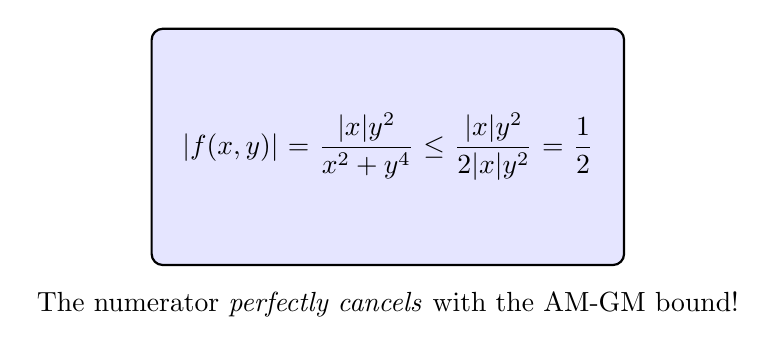
\begin{tikzpicture}[scale=1]
    \draw[thick, rounded corners, fill=blue!10] (-3, -1.5) rectangle (3, 1.5);
    \node[text width=5.5cm, align=center] at (0, 0) {
        $|f(x,y)| = \dfrac{|x| y^2}{x^2 + y^4} \leq \dfrac{|x| y^2}{2|x| y^2} = \dfrac{1}{2}$
    };
    \node at (0, -2) {The numerator \emph{perfectly cancels} with the AM-GM bound!};
\end{tikzpicture}
\end{center}

\subsection{Why Doesn't This Work for $g$?}

For $g$, the denominator is $x^2 + y^6$. AM-GM gives $x^2 + y^6 \geq 2|x|y^3$, so:
\[
|g(x,y)| \leq \frac{|x|y^2}{2|x|y^3} = \frac{1}{2|y|}
\]
This blows up as $y \to 0$! The AM-GM bound is not enough to control $g$.

\section{Part 2: Why is $g$ Unbounded Near the Origin?}

The key idea: approach $(0,0)$ along a \textbf{curve}, not a line.

\begin{center}
\begin{tikzpicture}[scale=1.5]
    \draw[->] (-0.5, 0) -- (2, 0) node[right] {$x$};
    \draw[->] (0, -1.5) -- (0, 1.5) node[above] {$y$};

    % The curve x = y^3
    \draw[red, thick, domain=-1.2:1.2, samples=50] plot ({\x*\x*\x}, \x);
    \node[red] at (1.8, 1.2) {$x = y^3$};

    % Show points approaching origin
    \foreach \y in {0.3, 0.5, 0.7, 0.9, 1.1} {
        \pgfmathsetmacro{\x}{\y*\y*\y}
        \fill[blue] (\x, \y) circle (1.5pt);
    }

    \node[text width=5cm, align=center] at (1, -2) {
        Along $x = y^3$:\\
        $g(y^3, y) = \dfrac{y^5}{2y^6} = \dfrac{1}{2y} \to \infty$
    };
\end{tikzpicture}
\end{center}

\textbf{Why does this work?} On the curve $x = y^3$, the two terms in the denominator become \emph{equal}: $x^2 = y^6$. This is the ``worst case'' --- the denominator is as small as possible relative to the numerator.

\section{Part 3: Why is $f$ Not Continuous at $(0,0)$?}

Same idea, but now use the parabola $x = y^2$ for $f$:

\begin{center}
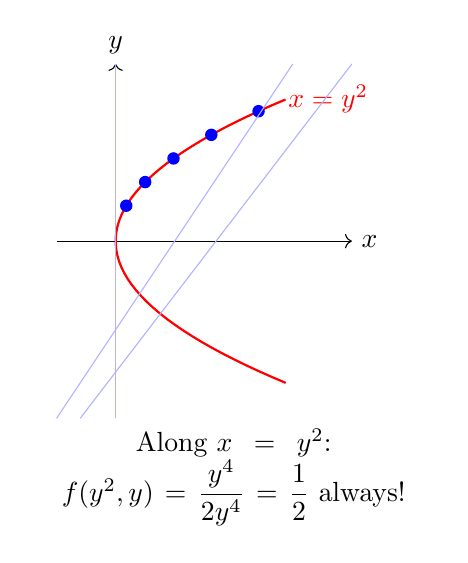
\begin{tikzpicture}[scale=1.5]
    \draw[->] (-0.5, 0) -- (2, 0) node[right] {$x$};
    \draw[->] (0, -1.5) -- (0, 1.5) node[above] {$y$};

    % The parabola x = y^2
    \draw[red, thick, domain=-1.2:1.2, samples=50] plot ({\x*\x}, \x);
    \node[red] at (1.8, 1.2) {$x = y^2$};

    % Show points approaching origin
    \foreach \y in {0.3, 0.5, 0.7, 0.9, 1.1} {
        \pgfmathsetmacro{\x}{\y*\y}
        \fill[blue] (\x, \y) circle (1.5pt);
    }

    % Lines through origin
    \draw[blue!30, thin] (-0.5, -1.5) -- (1.5, 1.5);
    \draw[blue!30, thin] (-0.3, -1.5) -- (2, 1.5);
    \draw[blue!30, thin] (0, -1.5) -- (0, 1.5);

    \node[text width=5cm, align=center] at (1, -2) {
        Along $x = y^2$:\\
        $f(y^2, y) = \dfrac{y^4}{2y^4} = \dfrac{1}{2}$ always!
    };
\end{tikzpicture}
\end{center}

On the parabola $x = y^2$, the denominator terms become equal: $x^2 = y^4$. So $f = \frac{y^4}{2y^4} = \frac{1}{2}$ everywhere on this curve. Since $f(0,0) = 0 \neq 1/2$, the function is not continuous at the origin.

\section{Part 4: Why Are Line Restrictions Continuous?}

\subsection{Lines Not Through the Origin}

Away from $(0,0)$, both $f$ and $g$ are ratios of polynomials with nonzero denominators. Rational functions are continuous wherever their denominators don't vanish.

\subsection{Lines Through the Origin}

On a line $y = mx$ (with $m \neq 0$), substitute:

\begin{center}
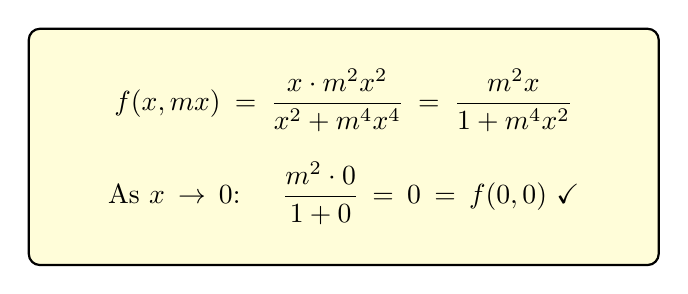
\begin{tikzpicture}
    \draw[thick, rounded corners, fill=yellow!15] (-4, -1.5) rectangle (4, 1.5);
    \node[text width=7cm, align=center] at (0, 0) {
        $f(x, mx) = \dfrac{x \cdot m^2 x^2}{x^2 + m^4 x^4} = \dfrac{m^2 x}{1 + m^4 x^2}$\\[1em]
        As $x \to 0$: \quad $\dfrac{m^2 \cdot 0}{1 + 0} = 0 = f(0,0)$ \checkmark
    };
\end{tikzpicture}
\end{center}

\textbf{The crucial point:} On any line $y = mx$, the substitution reduces the function to a nice rational function of one variable that equals $0$ at the origin. The ``dangerous'' behavior only appears along \emph{curves} (like $x = y^2$), never along \emph{lines}.

\subsection{Why Lines Miss the Problem}

\begin{center}
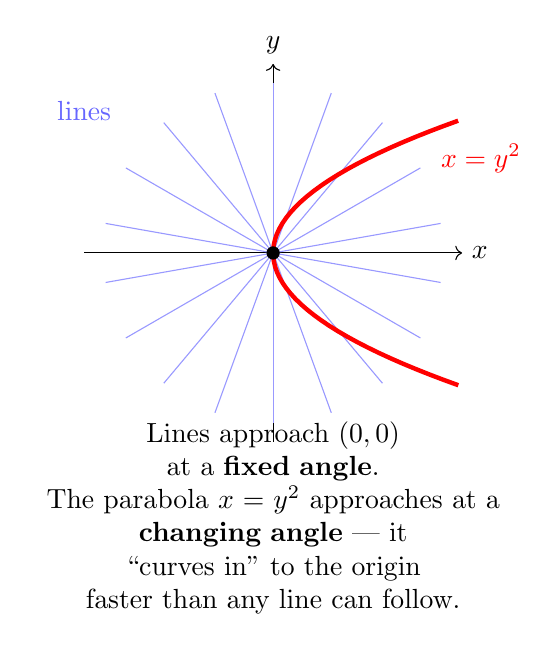
\begin{tikzpicture}[scale=1.2]
    \draw[->] (-2, 0) -- (2, 0) node[right] {$x$};
    \draw[->] (0, -2) -- (0, 2) node[above] {$y$};

    % Lines through origin
    \foreach \angle in {10, 30, 50, 70, 90, 110, 130, 150, 170} {
        \draw[blue!40] ({-1.8*cos(\angle)}, {-1.8*sin(\angle)}) -- ({1.8*cos(\angle)}, {1.8*sin(\angle)});
    }

    % Parabola
    \draw[red, ultra thick, domain=-1.4:1.4, samples=50] plot ({\x*\x}, \x);

    \fill (0,0) circle (2pt);

    \node[red] at (2.2, 1) {$x = y^2$};
    \node[blue!60] at (-2, 1.5) {lines};

    \node[text width=6cm, align=center] at (0, -2.8) {
        Lines approach $(0,0)$ at a \textbf{fixed angle}.\\
        The parabola $x = y^2$ approaches at a\\
        \textbf{changing angle} --- it ``curves in'' to the origin\\
        faster than any line can follow.
    };
\end{tikzpicture}
\end{center}

\textbf{On any fixed line} $y = mx$: the variable $x$ controls both coordinates, and $f$ simplifies to something well-behaved.

\textbf{On the parabola} $x = y^2$: the relationship between $x$ and $y$ is nonlinear, which ``matches the degree'' of the denominator and creates a constant value.

\section{Degree Matching: The Deep Reason}

Look at the degrees in $f = \frac{xy^2}{x^2 + y^4}$:
\begin{itemize}
    \item Numerator: $xy^2$ has ``weighted degree'' $1 + 2 = 3$ (if $x$ counts as 2, $y$ as 1)
    \item Actually, think of it as: if $x \sim y^2$, then $xy^2 \sim y^4$ and $x^2 + y^4 \sim 2y^4$
    \item So $f \sim y^4/(2y^4) = 1/2$ --- a nonzero constant!
\end{itemize}

On a line $y = mx$: $x \sim x$ (not $\sim y^2$), so the degrees \emph{don't} match, and $f \to 0$.

The parabola $x = y^2$ is the exact curve where the degrees balance, creating a nonzero limit.

\end{document}
